\documentclass[12pt]{article}

\usepackage{amsmath}
\usepackage{geometry}
\usepackage{graphicx}
\usepackage{setspace}
\usepackage{float}
\usepackage{subcaption}

\geometry{margin=1in}
\setstretch{1.2}

\title{Modeling Global Energy Crisis Cascades using Complexity Science}
\author{Entry Number: 2023CH10882 \\ Name: Manya Agrawal}
\date{\today}

\begin{document}

\maketitle

\tableofcontents
\newpage

\begin{abstract}
The global energy system is undergoing rapid transformation driven by geopolitical instability, the transition toward electric vehicles (EVs), and increasing dependence on critical minerals such as lithium and cobalt. These interacting subsystems form a highly interconnected and nonlinear network that exhibits characteristics of complex systems. In this study, we model global energy networks using tools from complexity science to analyze cascading failures arising from localized disruptions. By incorporating stochastic disturbances, network connectivity, and threshold dynamics, we demonstrate the emergence of avalanche-like failures. The simulations show that avalanche sizes range from frequent small failures to rare large cascades, indicating approximate power-law behavior over intermediate scales. Furthermore, we compare oil-dominated and EV-mineral-based networks to highlight the role of connectivity in structural vulnerability. The results indicate that global energy systems may operate near a self-organized critical state, where small perturbations can trigger disproportionately large disruptions.
\end{abstract}

\section{Introduction}

The modern global energy system is one of the most complex engineered systems in existence. It encompasses oil production networks, electricity grids, and increasingly, supply chains for critical minerals required in renewable technologies and electric vehicles (EVs). Recent global developments, including geopolitical conflicts, supply chain disruptions, and rapid technological transitions, have exposed the inherent fragility of these systems.

Traditional engineering approaches often assume linearity and predictability. However, real-world energy systems display nonlinear interactions, feedback loops, and emergent behavior. For instance, a disruption in oil supply in one region can propagate through international trade networks, affecting fuel prices, electricity generation, and industrial production worldwide. Similarly, increased demand for EVs places stress on mineral supply chains, potentially triggering cascading shortages.

Such phenomena cannot be adequately explained using reductionist frameworks. Instead, complexity science provides a powerful lens to study these systems by focusing on interactions, network structures, and emergent collective behavior.

\section{4a. Why the System is a Good Candidate for Complexity Science}

The global energy system satisfies all defining characteristics of a complex system.

Firstly, it consists of a large number of interacting agents, including countries, corporations, and industrial sectors. Each agent operates based on local objectives but is constrained by global interactions. These interactions are not merely additive but nonlinear, meaning that small changes in one part of the system can produce disproportionately large effects elsewhere.

Secondly, the system is subject to stochastic disturbances, or noise. These disturbances arise from unpredictable events such as geopolitical conflicts, natural disasters, policy changes, and fluctuations in market demand. Such randomness plays a critical role in driving system dynamics.

Thirdly, the system exhibits emergent behavior. Global energy crises do not originate from a single centralized failure but emerge from the accumulation and propagation of local disruptions.

Finally, the system is structured as a network with heterogeneous connectivity. Some nodes act as hubs with a large number of connections, while others are sparsely connected. This heterogeneity significantly influences system stability and failure propagation.

These features collectively make the global energy system an ideal candidate for analysis using complexity science, particularly in the context of self-organized criticality and avalanche dynamics.

\section{4b. System Description: Noise, Avalanche, and Connectivity}

In the present model, the system is represented as a network where nodes correspond to countries or industrial entities, and edges represent trade relationships involving energy resources.

\subsection*{Connectivity}

Connectivity defines how nodes are linked through trade. In oil networks, connectivity is typically scale-free, meaning a few major exporters or hubs dominate global supply. In contrast, EV mineral networks are modeled as more randomly connected systems, representing a comparatively distributed supply structure.

The degree of a node, defined as the number of connections it has, determines its influence. Highly connected nodes play a crucial role in maintaining system stability but also represent points of vulnerability.

\subsection*{Noise}

Noise is introduced as random perturbations in resource availability. These perturbations simulate real-world uncertainties such as production cuts, geopolitical tensions, policy changes, natural disasters, or sudden demand surges. Noise acts as the driving force that pushes the system toward instability.

\subsection*{Avalanche Dynamics}

An avalanche is defined as a cascading failure triggered by a local disruption. When a node experiences a resource deficit below a critical threshold, it fails to meet its obligations, reducing supply reliability for connected nodes. This initiates a chain reaction where neighboring nodes also experience stress and may subsequently fail.

The size of an avalanche is quantified as the total number of nodes affected during this cascade. Avalanches can range from small localized failures to large-scale systemic crises.

\section{4c. Computer Simulation}

The system is modeled using network theory, where a graph $G(N,E)$ represents the global energy network. In this graph, nodes represent countries or energy sectors, while edges represent energy trade or supply-chain dependence.

Two network structures are compared:

\begin{itemize}
    \item \textbf{Oil-dominated network:} modeled as a scale-free network using the Barabási--Albert model.
    \item \textbf{EV-mineral network:} modeled as a random network using the Erdős--Rényi model.
\end{itemize}

Each node is assigned a resource level $R_i$, representing its capacity to meet demand. A random node is subjected to a shock, reducing its resource level. If the resource level falls below a critical threshold, the node fails. This failure then propagates stress to neighboring nodes.

The stress propagation is modeled as:

\[
R_j \leftarrow R_j - \Delta \cdot \frac{1}{\sqrt{1+k_j}}
\]

where $R_j$ is the resource level of neighboring node $j$, $\Delta$ is the propagation loss, and $k_j$ is the degree of node $j$. The factor $\frac{1}{\sqrt{1+k_j}}$ prevents immediate collapse of the entire network while still allowing failures to propagate through connected nodes.

The simulation proceeds as follows:

\begin{itemize}
    \item A network is generated using either a scale-free model or a random graph model.
    \item Each node is initialized with a random resource level.
    \item A random node is subjected to a shock.
    \item If the resource level falls below a threshold, the node fails.
    \item Failure propagates to neighboring nodes by reducing their resource levels.
    \item The process continues iteratively until no new failures occur.
    \item The total number of failed nodes is recorded as the avalanche size.
\end{itemize}

\begin{figure}[H]
\centering
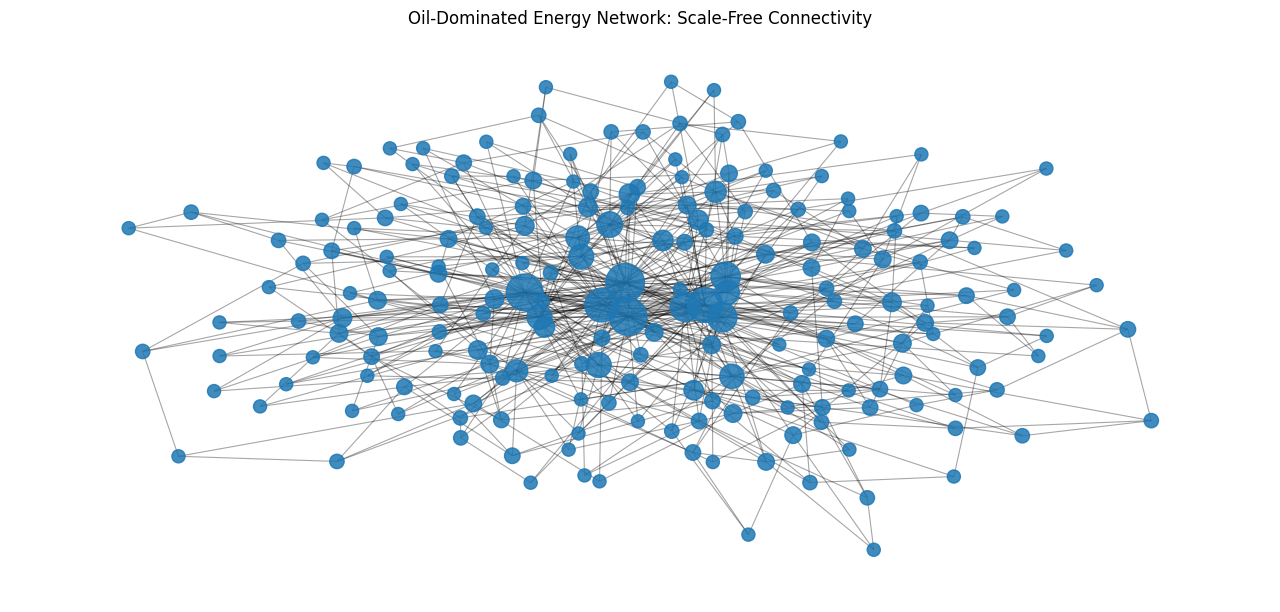
\includegraphics[width=0.82\textwidth]{graph1_oil_scale_free_network.png}
\caption{Oil-dominated energy network modeled as a scale-free network. Larger nodes indicate higher connectivity. The presence of hub nodes reflects the concentrated structure of oil supply systems.}
\end{figure}

\begin{figure}[H]
\centering
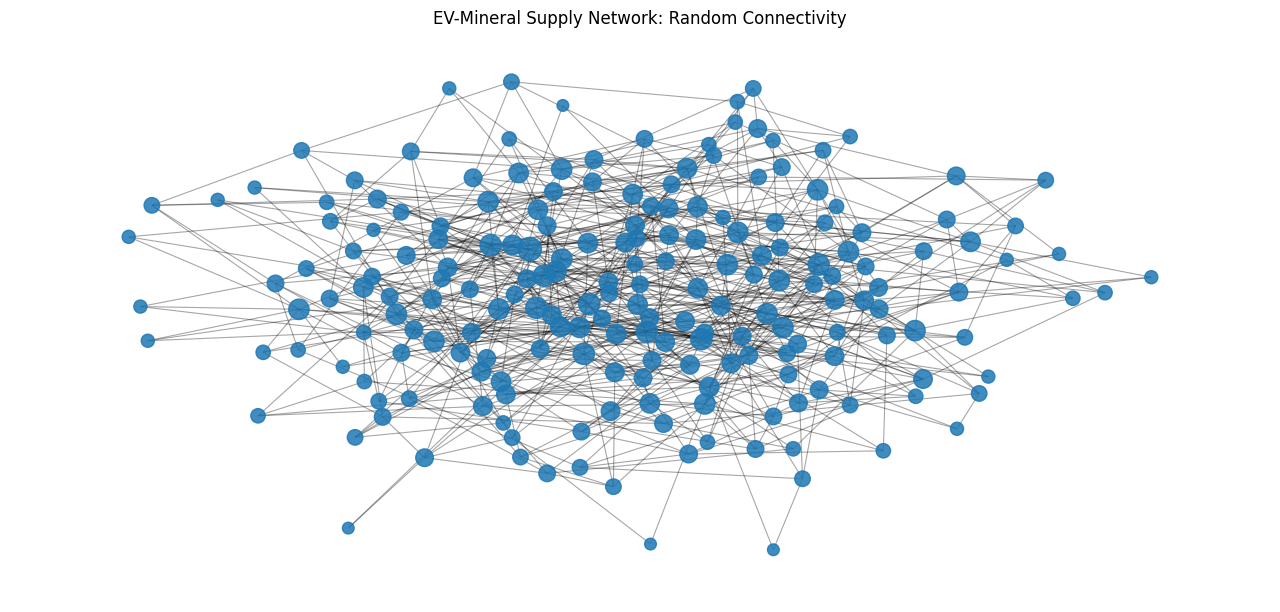
\includegraphics[width=0.82\textwidth]{graph2_ev_random_network.png}
\caption{EV-mineral supply network modeled as a random network. The connectivity is more uniformly distributed compared to the oil-dominated network.}
\end{figure}

\section{4d. Analysis of Avalanche Distribution and Connectivity}

The statistical distribution of avalanche sizes was analyzed over multiple simulation runs. The results show a broad range of avalanche sizes, from very small cascades to large events affecting a significant fraction of the network.

The avalanche size distribution is expected to follow an approximate power-law relation:

\[
P(s) \propto s^{-\alpha}
\]

where $P(s)$ is the probability or frequency of an avalanche of size $s$, and $\alpha$ is the power-law exponent.

\begin{figure}[H]
\centering
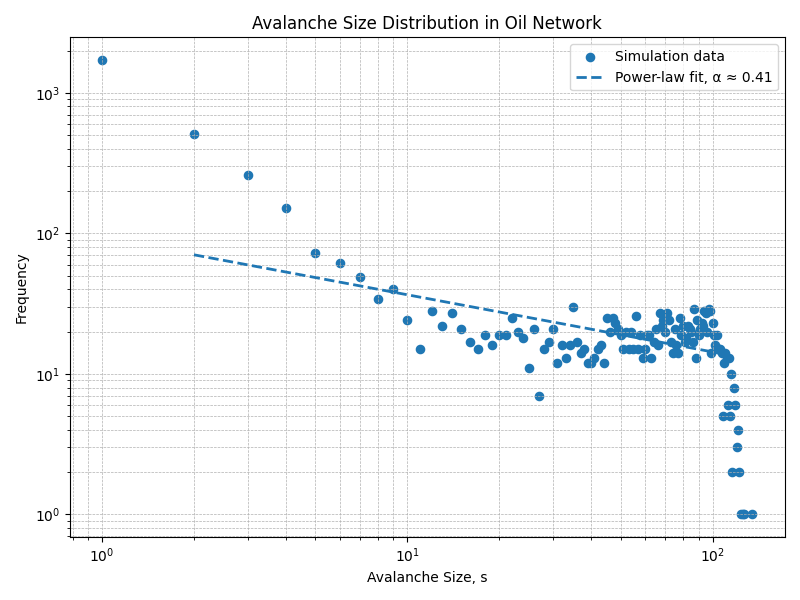
\includegraphics[width=0.82\textwidth]{graph3_oil_avalanche_distribution.png}
\caption{Avalanche size distribution for the oil-dominated scale-free network. Small avalanches occur frequently, while large avalanches occur rarely. The approximate linear region in the log-log plot suggests approximate power-law scaling over intermediate ranges.}
\end{figure}

\begin{figure}[H]
\centering
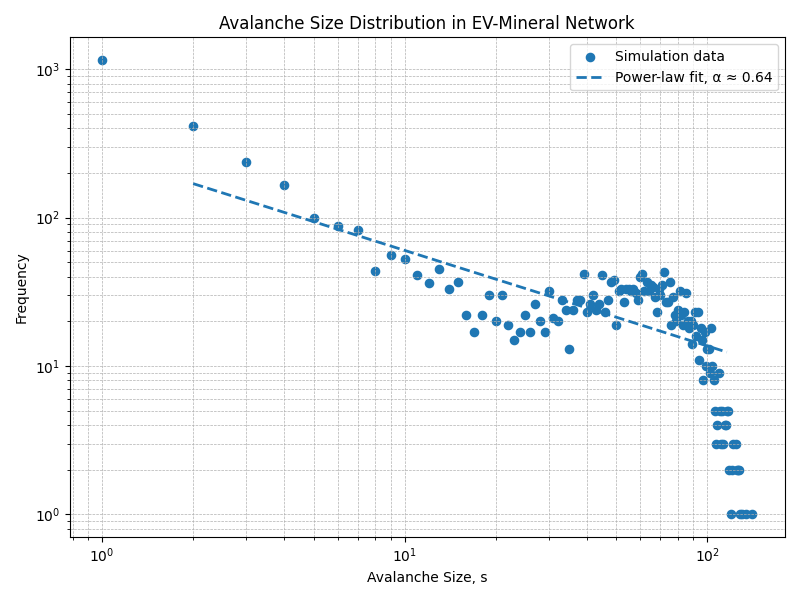
\includegraphics[width=0.82\textwidth]{graph4_ev_avalanche_distribution.png}
\caption{Avalanche size distribution for the EV-mineral random network. The distribution also shows frequent small avalanches and rarer large events, indicating cascading behavior in the random network.}
\end{figure}

The log-log plots exhibit approximately decreasing trends over intermediate avalanche sizes. This supports the presence of power-law-like behavior, although deviations occur at large avalanche sizes due to finite system size effects. Since the simulated network contains a fixed number of nodes, the avalanche size cannot grow indefinitely, causing the tail of the distribution to bend downward.

A key observation is the strong dependence of avalanche behavior on network connectivity. In the scale-free oil network, highly connected hub nodes participate in cascading failures and can amplify systemic risk. In the random EV-mineral network, failures are more distributed across nodes of moderate connectivity.

\begin{figure}[H]
\centering
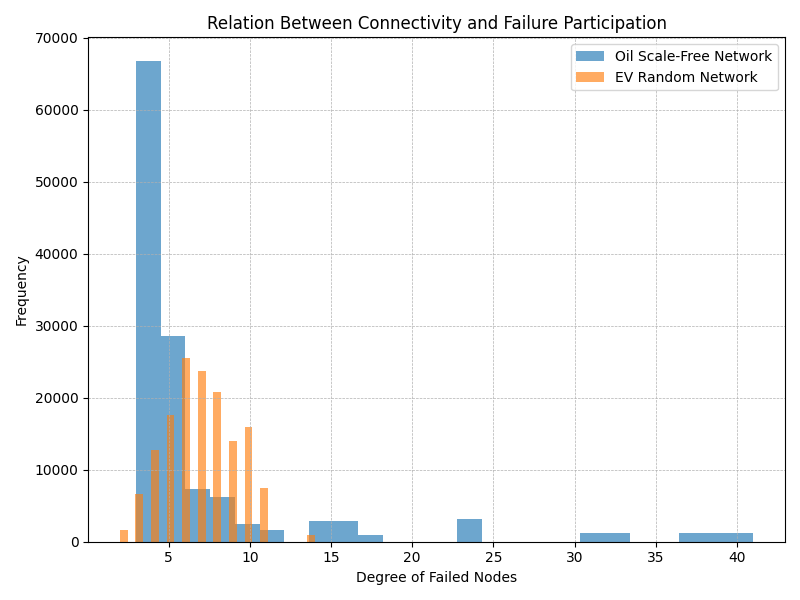
\includegraphics[width=0.82\textwidth]{graph5_connectivity_vs_failure.png}
\caption{Relation between connectivity and failure participation. The oil-dominated scale-free network shows a long tail, indicating that high-degree hub nodes participate in failures. The EV-mineral network shows a more concentrated failure pattern.}
\end{figure}

Thus, connectivity plays a dual role. Under normal conditions, high connectivity improves efficiency and resource flow. However, during disruptions, the same connectivity can amplify cascading failures.

\section{4e. Self-Organized Criticality}

The simulation results demonstrate key features of self-organized criticality. In a self-organized critical state, the system remains near the boundary between stability and instability. Small perturbations may dissipate locally, while some disturbances may escalate into large-scale cascades.

\begin{figure}[H]
\centering
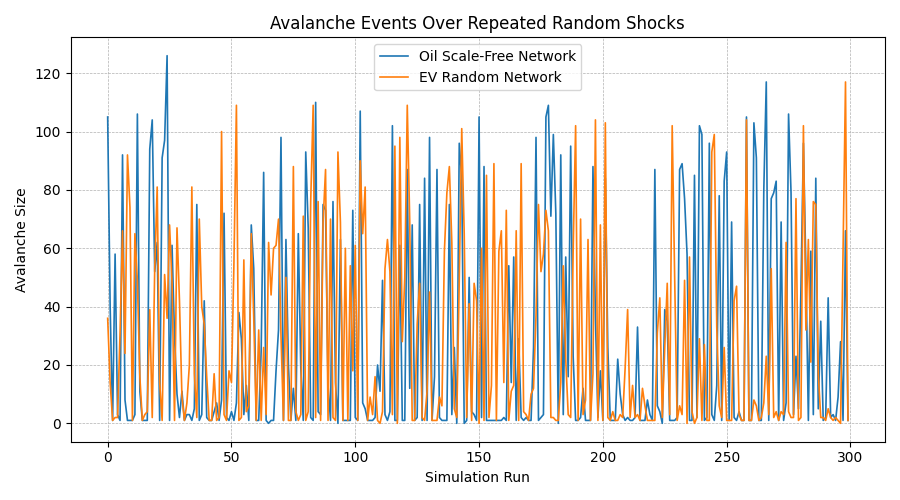
\includegraphics[width=0.82\textwidth]{graph7_avalanche_time_series.png}
\caption{Avalanche sizes over repeated random shocks. The time series shows intermittent spikes, where large cascades occur suddenly among many smaller events. This is characteristic of systems operating near a critical state.}
\end{figure}

The time series shows irregular bursts of large avalanche events interspersed with many smaller events. This behavior indicates that large crises are not isolated anomalies but may arise naturally from the internal dynamics of the interconnected energy network.

The avalanche size distributions also support this interpretation. Small avalanches are common, medium avalanches occur occasionally, and large avalanches are rare but significant. This absence of a single typical avalanche size is consistent with self-organized criticality.

These observations indicate that the system self-organizes near a critical point without the need for external tuning of parameters.

\section{Comparison of Network Behavior}

\begin{figure}[H]
\centering
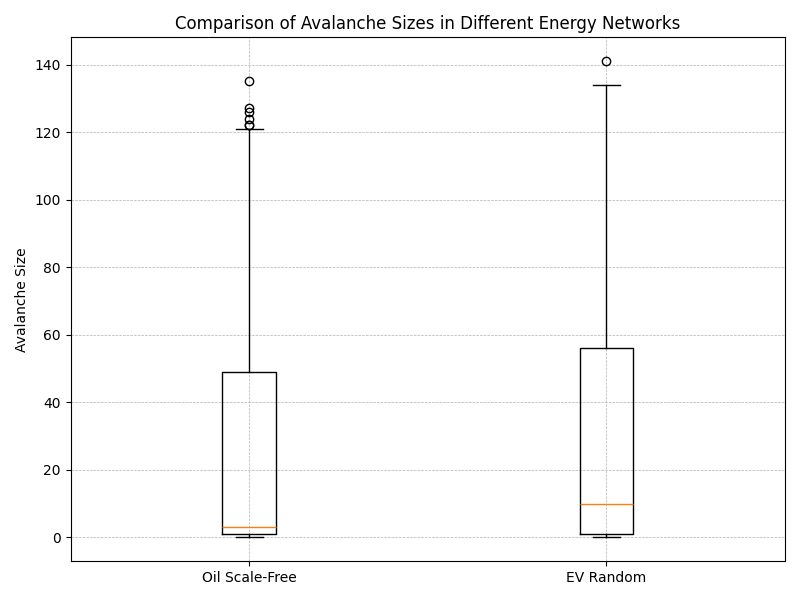
\includegraphics[width=0.82\textwidth]{graph6_avalanche_comparison.png}
\caption{Comparison of avalanche sizes in the oil-dominated scale-free network and the EV-mineral random network. Both networks show broad avalanche behavior, but the scale-free network exhibits strong hub-driven vulnerability.}
\end{figure}

The comparison shows that both energy networks are vulnerable to cascading failures, but the mechanism of vulnerability differs. The oil-dominated network is vulnerable because highly connected hubs can transmit stress to many other nodes. The EV-mineral network, while more uniformly connected, can still experience large avalanches due to distributed stress propagation.

Therefore, diversification alone may not eliminate systemic risk. Resilience requires both reduced dependence on hubs and improved management of distributed supply-chain vulnerabilities.

\section{Discussion}

The findings of this study have significant implications for energy policy and infrastructure design. The dominance of hub nodes in oil networks suggests a need for diversification to reduce systemic risk. If a major hub fails, the resulting cascade can affect many connected regions.

The growing reliance on critical minerals for EV technologies introduces a different type of vulnerability. Although the EV-mineral network is modeled as more randomly connected, it still exhibits cascading failures. This suggests that future energy systems must account not only for direct resource availability but also for the structure of interdependence.

The results also highlight the importance of monitoring critical nodes and links. Identifying nodes with high degree or high participation in avalanches can help policymakers and planners design more resilient energy networks.

From a complexity science perspective, the study shows how large-scale crises can emerge from simple local rules: random shocks, threshold failure, and stress propagation. This supports the argument that energy crises are systemic phenomena rather than isolated events.

\section{Conclusion}

This study demonstrates that global energy systems exhibit complex dynamics governed by noise, connectivity, and nonlinear interactions. The emergence of avalanche behavior and power-law-like distributions indicates that the system may operate near a self-organized critical state.

A key finding is the role of network structure in shaping vulnerability. Scale-free oil-dominated networks are efficient but fragile because of their reliance on hub nodes. Random EV-mineral networks distribute connections more evenly but remain susceptible to cascading failures under repeated shocks.

The simulation results show that small avalanches occur frequently, medium avalanches occur occasionally, and large avalanches occur rarely. This pattern is characteristic of systems near criticality. Deviations from perfect power-law behavior are expected due to finite network size and stochastic variation.

Understanding these dynamics is essential for designing resilient energy systems capable of withstanding future disruptions. Complexity science provides a valuable framework for analyzing systemic risk and guiding future energy infrastructure planning.

\section{Prompts Used}

The following prompts were used during the preparation of this project:

\begin{itemize}
    \item Explain why global energy crisis cascades are suitable for complexity science.
    \item Provide Python code for simulating avalanche dynamics in energy networks.
    \item Help me interpret whether my simulation graphs show self-organized criticality.
\end{itemize}

\section{Code and Repository}

The Python simulation code, generated graphs, LaTeX source file, PDF report, and supporting documents are stored in a Git-based repository.

\textbf{GitHub Link:} https://github.com/Manya070/complexity-social-network-cascade


\section{Acknowledgement of Help}

I would like to express my sincere gratitude to Prof. Rajesh Khanna for his guidance and for teaching the course on Complexity Science, which provided the foundational understanding required for this project.

Assistance was taken from an AI agent for conceptualizing the project topic, designing the simulation framework, debugging the Python code, interpreting results, and preparing the LaTeX report. The final understanding, verification, and submission are the responsibility of the author.

\end{document}